\chapter{AutoAFIDs: Automatic Anatomical Fiducial Localization} \label{chap:AutoAFIDs}
\newpage
\sloppy
This chapter is largely based on:
\begin{itemize}[noitemsep,topsep=0pt]
    \item {\small A. Taha, M. Abbass, D. Bansal, M. Snyder, A. Thurairajah, T. Kuehn, J. Kai, M. Salman, G. Gilmore, A.R. Khan, J.C. Lau.} AutoAFIDs: Automatic brain landmark detection for quality control, stereotactic targeting, and brain charting. \textit{In Preparation}.
\end{itemize}


\section{Introduction}
\subsection{Brain Coordinates in Neuroimaging and Neurosurgery}
Three-dimensional Cartesian coordinates (x, y, z) offer a convenient and precise framework to represent brain structures. This abstraction underlies a broad range of applications in both neuroimaging and neurosurgical workflows, enabling reproducibility \cite{Dockes2020-nw}, cross-subject comparison \cite{Glasser2016-ko}, and multimodal data integration \cite{Uludag2014-qz}. In research, coordinates form the backbone of meta-analytic platforms such as \texttt{NeuroSynth} \cite{Yarkoni2011-sr} and \texttt{NeuroQuery} \cite{Dockes2020-nw}, which aggregate reported coordinates from thousands of studies to identify consistent associations between brain and behavior. In clinical contexts, neuromodulation targets and optimal stimulation zones are represented by coordinates relative to the major anatomical landmarks \cite{Horn2017-bi} such as anterior and posterior commissure (AC and PC), guiding trajectory planning and enabling retrospective outcome analysis. Across both domains, coordinates are a shared spatial language for modeling and navigating the brain.

\subsection{Automatic Landmark Localization}
The manual localization of brain landmarks is often time-intensive, cognitively demanding, and subject to inter-rater variability \cite{Abbass2022-lf, Lau2019-eh,Pallavaram2008-zr}. Even with detailed annotation protocols, raters typically require training to achieve consistency \cite{Lau2019-eh}. These challenges pose a barrier to scaling coordinate-based workflows across large datasets and neuroimaging pipelines. To address this bottleneck, deep learning (DL) methods offer a promising avenue for automatic landmark detection in brain MRI. DL-based approaches typically fall into two paradigms: (1) coordinate regression \cite{Neupane2024-vt} and (2) heatmap-based localization \cite{Payer2016-ik}. In coordinate regression, a network directly outputs the x,y,z coordinates of each target (i.e., landmark) often via fully connected layers or global pooling. In heatmap-based methods, the network predicts a probability map---often a Gaussian “fuzzy” blob---for each landmark and the peak of the heatmap is taken as the location. Heatmap regression has become especially popular because it retains spatial context and enables designing the network to localize landmarks in a fully convolutional manner.

\subsection{Deep Learning Approaches}
DL has significantly advanced the field of computer vision by enabling end-to-end learning of hierarchical features directly from data, leading to substantial improvements in tasks such as facial landmark detection, pose estimation, and image registration \cite{Lathuiliere2018-oy}. While medical imaging adopted these tools more gradually, fully convolutional networks—particularly U-Net and its 3D variants—have since become foundational for segmentation and anatomical localization tasks \cite{Akkus2017-eh, Falk2019-us}. Variants such as V-Net and cascaded U-Nets improve spatial precision by capturing both global context and local detail, while architectures like the spatial configuration network (SCN) \cite{Payer2016-ik, Payer2019-sn} and multi-task cascaded CNNs \cite{Zhang2017-dc} embed geometric priors to enhance performance in data-scarce settings. More recently, self-configuring pipelines like nnLandmark \cite{Ertl2025-wu} and attention-based models such as H3DE-Net \cite{Huang2025-vt} have streamlined deployment and improved model efficiency. Despite these advances, relatively limited studies have adapted such innovations to the detection of brain landmarks central to stereotactic targeting and coordinate-based neuroimaging \cite{Edwards2021-su}. Given their consistent anatomy and clinical importance, AC-PC detection represents a promising use case for applying modern deep learning techniques to improve automation, reproducibility, and standardization in brain mapping workflows.

\subsection{Limitations in the field}
Several barriers limit the broader utility of these DL techniques. First, well-annotated, publicly available datasets with standardized brain landmarks remain scarce, which constrains training, benchmarking, and validation. Second, many existing models are not open-source, are difficult to reproduce, or lack adherence to FAIR (Findable, Accessible, Interoperable, and Reusable; \cite{Wilkinson2016-it}) data principles. Third, to the best of our knowledge, no automated workflows are built in environments compatible with the Brain Imaging Data Structure (BIDS; (Gorgolewski et al., 2016)), which impedes integration with modern neuroimaging pipelines and limits accessibility for the broader scientific community. As a result, the full potential of automated coordinate-based analysis for applications such as registration quality control, brain morphometry, or lifespan brain charting remains underrealized.

\subsection{Our Proposed Approach}
In this work, we present \texttt{AutoAFIDs}, a BIDS-App for automatic landmark detection using deep learning. We trained and tested \texttt{AutoAFIDs} using a curated open-access dataset of MRI scans (n = 202) across a range of MRI field strengths (1.5, 3, and 7T) and conditions (healthy, abnormal ventricles, and neurodegenerative) with 20,000+ landmarks manually localized by human raters. \texttt{AutoAFIDs} demonstrated a landmark localization accuracy comparable to human raters. We also demonstrate the broad utility of \texttt{AutoAFIDs} for two downstream applications which we make available to end-users: 1) quality control of image registration, 2) stereotactic target localization. By applying \texttt{AutoAFIDs} on over 2,000 MRI scans from individuals aged 18 to 100, we uncovered millimetric differences in brain structure that distinguish healthy brain changes from early signs of neurodegenerative disease.

\section{Methods}
\subsection{Problem Definition}
\label{sec:problemstatement}
The objective of this study was to localize anatomical fiducial points distributed across multiple brain regions using a supervised deep learning framework. Let $\mathcal{V} \subset \mathbb{R}^3$ denote a 3D brain volume, and let $\{p_1, p_2, \ldots, p_L\}$ represent the set of $L$ target landmark coordinates, where each $p_\ell \in \mathbb{R}^3$ denotes the location of the $\ell^{\text{th}}$ anatomical point of interest.

We formulated this as a regression problem in which the model learns to predict a smooth, continuous-valued distance map centered on the target landmark. For each voxel $v \in \mathcal{V}$ and landmark $\ell$, the ground truth target $D^\ell(v)$ is defined as:

\begin{equation}
D^\ell(v) = \lVert v - p_\ell \rVert_2
\end{equation}

To enhance stability and spatial resolution, we applied an exponential decay to the predicted distance map:

\begin{equation}
T^\ell(v) = \exp(-\alpha \cdot D^\ell(v))
\end{equation}

where $\alpha$ is a fixed scaling factor controlling the spatial decay rate. During training, the model learns to predict this transformed image using a mean squared error (MSE) loss between the predicted image \( \hat{T}(v) \) and the ground-truth target \( T(v) \) across all voxels \( v \) in the prediction region \( \mathcal{V} \):

\begin{equation}
\mathcal{L} = \frac{1}{|\mathcal{V}|} \sum_{v \in \mathcal{V}} \left( \hat{T}(v) - T(v) \right)^2
\end{equation}

Here, \( \mathcal{V} \) denotes the set of voxels within the input patch or volume, \( T(v) \) is the ground-truth voxelwise signal derived from the known landmark coordinate, and \( \hat{T}(v) \) is the model’s prediction at voxel \( v \). This formulation enables dense supervision and encourages the model to produce spatially coherent predictions with millimetric localization accuracy.


\subsection{Imaging and Coordinate Data}

We made use of landmarks defined by the Anatomical Fiducials (AFIDs) protocol, a standardized set of 32 brain landmarks manually placed on structural T1-weighted MRI scans \cite{Lau2019-eh}. These fiducials span diverse anatomical regions, including subcortical nuclei, ventricular boundaries, and midline structures such as the anterior and posterior commissures. The imaging acquisition protocols, annotation procedures, and coordinate data used here are described in detail in Chapter~\ref{chap:afidsdata} but shown in Figure \ref{fig:ch3_Figure_data} for completeness.

For model development, all curated datasets were divided into training ($n = \textbf{148}$), validation ($n = \textbf{42}$), and testing ($n = \textbf{21}$) subsets. Stratified splitting of each dataset was used to ensure representative anatomical and demographic diversity across all sets.

\begin{figure}[hbt!]
    \centering
    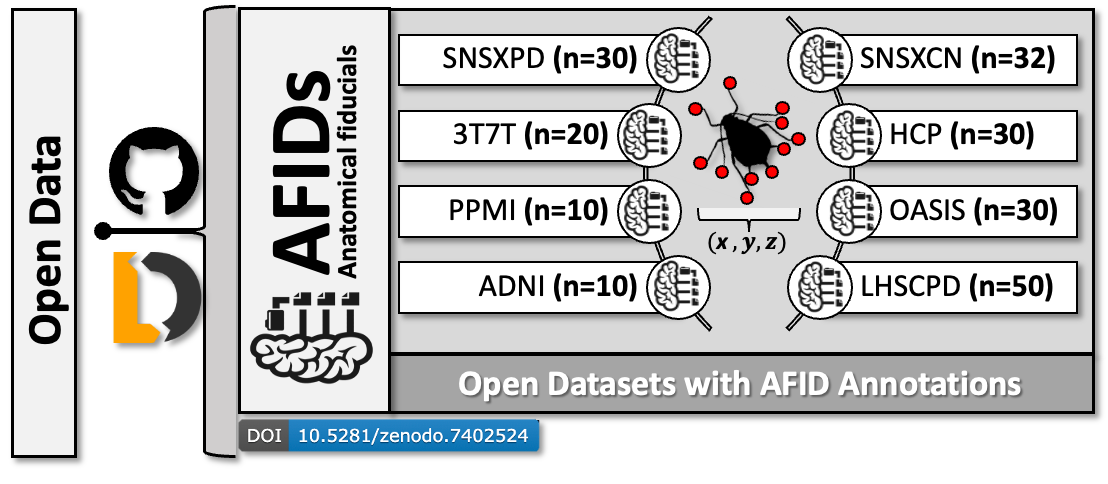
\includegraphics[width=1\linewidth]{figs/ch3_Figure_data.png}
    \caption{We made use of a previously released dataset containing anatomical fiducial (AFID) annotations. This dataset comprises eight sub-datasets spanning a range of MRI field strengths and neurodegenerative conditions. For machine learning modeling, we apply a stratified 70/20/10 split into training, validation, and test sets. By training on the combined heterogeneous dataset, the model is encouraged to learn features that are agnostic to imaging resolution, field strength, and MRI acquisition parameter differences.}
    \label{fig:ch3_Figure_data}
\end{figure}

\subsection{Preprocessing and Data Preparation}

We adopted standardized preprocessing profiles inspired by the nnU-Net framework \cite{Isensee2021-ev}, with additional modifications tailored for anatomical landmark detection. We built our workflow with Snakemake \cite{Koster2012-ok} in a BIDS-compliant fashion (i.e., SnakeBIDS; \cite{Van-Dyken2025-cn}). Input data were T1-weighted (T1w) structural MRIs, optionally converted from alternate contrasts (e.g., T2w, FLAIR, CT) using SynthSR \cite{Iglesias2023-co} when specified. 

\begin{figure}[hbt!]
    \centering
    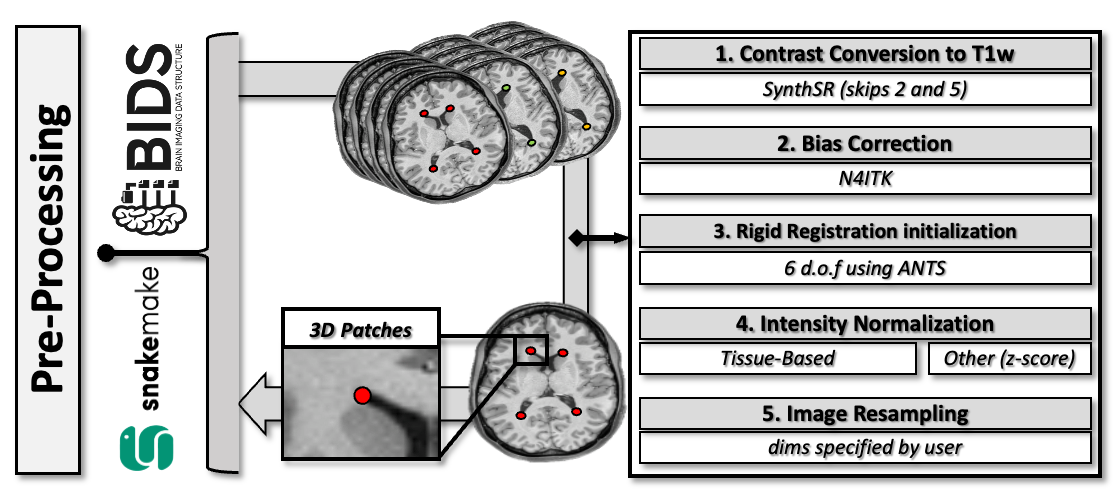
\includegraphics[width=1\linewidth]{figs/ch3_Figure_proc.png}
    \caption{Overall preprocessing pipeline employed in \texttt{AutoAFIDs}. Preprocessing is generally modality specific but centered around processing T1w MRI. We make use of (1) SynthSR \cite{Iglesias2023-co} to convert various modalities (e.g., T2w, CT, or FLAIR) to T1w image. Subsequently, a T1w image goes through the following preprocessing steps: (2) bias correction \cite{Tustison2010-qu}, (3) rigid registration of an annotated template for landmark priors, (4) MRI volume intensity normalization performed using various user-specified options and finally (5) resampling of the MRI volume to an isotropic resolution. The SynthSR model already outputs images that do not need to undergo preprocessing steps 2 and 5.}
    \label{fig:ch3_Figure_proc}
\end{figure}


All T1w MRI scans undergo the following steps:

\begin{enumerate}
    \item \textbf{Bias field correction:} N4 bias field correction \cite{Tustison2010-nw} is applied to mitigate intensity non-uniformities arising from scanner-related artifacts.
    
    \item \textbf{Intensity normalization:} Each MRI volume is independently z-score normalized by subtracting its mean intensity and dividing by its standard deviation. Optionally, min-max normalization to the \([0, 1]\) range is also supported.

    
    \item \textbf{Isotropic resampling:} All volumes are resampled to a uniform 1~mm isotropic resolution to ensure consistent spatial scaling across subjects.
    
    \item \textbf{Template-to-subject registration:} A rigid registration of the MNI152NLin2009cAsym template to each subject’s native space is performed using ANTs \cite{Avants2011-zs}. This transformation is applied only to restrict the inference search space and guide patch sampling, without altering anatomical label coordinates.
    
    \item \textbf{Patch extraction:} For each landmark, a 3D patch is extracted from the input volume, centered on its expected location. This localized strategy reduces memory demands and enables precise, landmark-specific localization.
    
    \item \textbf{Spatial augmentation:} During training, 3D patches are augmented via random rigid rotations. Each rotation is applied about a uniformly sampled axis with an angle drawn from a normal distribution with zero mean and standard deviation $\sigma_{\text{angle}}$ (in degrees), promoting rotational robustness.
\end{enumerate}

Ground-truth heatmaps for each landmark are generated by computing the voxel-wise Euclidean distance (ED) to the target coordinate and applying an exponential decay function as described in Section \ref{sec:problemstatement}.

\subsection{Patch-Based Inference}

Rather than processing the entire volume, the model predicts landmarks using a patch-based strategy. For each target landmark $\ell$, we extract a cubic patch of size $2r+1$ centered on a prior coordinate $p_\ell^{\text{prior}}$ obtained by registering a standard template (e.g., MNI space) to the subject’s native image. Let $\mathcal{P}_\ell$ denote the local patch centered on $p_\ell^{\text{prior}}$:

\begin{equation}
\mathcal{P}_\ell = \left\{ v \in \mathcal{V} \ \middle|\ \lVert v - p_\ell^{\text{prior}} \rVert_\infty \leq r \right\}
\end{equation}

The input to the network is a single-channel image patch, and the output is a distance map over $\mathcal{P}_\ell$. The predicted landmark $\hat{p}_\ell$ is extracted as the centroid of the thresholded exponential-transformed output:

\begin{equation}
\hat{p}_\ell = \text{centroid} \left( \left\{ v \in \mathcal{P}_\ell \ \middle|\ \exp(-\alpha \cdot \hat{D}^\ell(v)) > \tau \right\} \right)
\end{equation}

where $\tau$ is a percentile-based threshold (e.g., top 1\%) applied to suppress noisy responses and extract a coherent region.

\subsection{Model Architecture and Training}

Each landmark is predicted using a separate deep neural network trained independently. The shared architecture is a lightweight 3D U-Net implemented in TensorFlow. Training was performed using the Adam optimizer with early stopping on a validation set. The loss function is mean squared error between the predicted and target distance maps (after exponential transform), as described above.

\begin{figure}[hbt!]
    \centering
    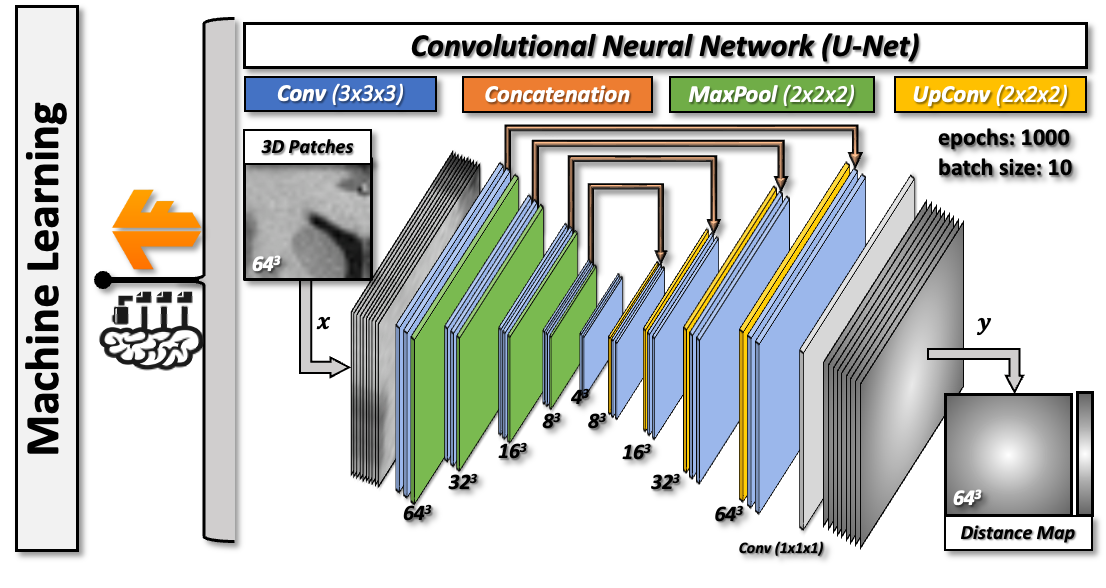
\includegraphics[width=1\linewidth]{figs/ch3_Figure_cnn.png}
    \caption{Overview of the deep learning model architecture used for anatomical fiducial localization. The model is a 3D U-Net that takes as input a 3D patch centered around a prior landmark location. The network consists of convolutional blocks (Conv, 3×3×3), downsampling via max-pooling (2×2×2), and upsampling via transposed convolutions (UpConv, 2×2×2). Skip connections concatenate encoder and decoder feature maps to preserve spatial detail. The output is a single-channel distance map representing the ED from each voxel to the target anatomical landmark.}
    \label{fig:ch3_Figure_cnn}
\end{figure}


\subsection{Model Design Rationale}
In this work, we adopt a one-network-per-landmark training strategy. While many existing approaches predict all landmarks jointly using a multi-channel output architecture, we opt for training separate models for each anatomical point. This decision is motivated by two key considerations. First, the anatomical heterogeneity of the landmarks poses a significant modeling challenge. The AFIDs span multiple tissue types and spatial contexts—including landmarks adjacent to ventricles, embedded within white matter tracts, and lying on cortical gray matter surfaces. These diverse appearance profiles often demand different spatial priors and texture sensitivities, which a shared model may struggle to learn simultaneously. Training distinct models allows each network to specialize in the local anatomical context of its assigned landmark, without interference from competing objectives. Second, certain use cases—such as deep brain stimulation (DBS)—require sub-voxel precision in landmark localization. Errors of just a few millimeters can lead to clinically significant deviations in surgical targeting or trajectory planning. In such high-stakes applications, even minor improvements in accuracy for individual landmarks can have meaningful downstream impact. By isolating each landmark into its own dedicated model, we maximize the opportunity for hyperparameter tuning, data augmentation, and architectural adaptation tailored to each target's anatomical and clinical importance. Together, these considerations justify a modular, per-landmark approach that prioritizes accuracy and adaptability over computational efficiency.

\section{Results}
\subsection{Landmark Localization Accuracy}
Model performance was evaluated on a held-out test set (n = 21) by computing the ED between predicted and ground truth AFID coordinates (see Figure \ref{fig:ch3_Figure_autoscore}). Across all 32 anatomical landmarks (672 predictions in total), the model achieved high spatial accuracy, with a median ED of 1.21 mm and an interquartile range (IQR) of 0.76–1.95 mm. 

\begin{figure}[hbt!]
    \centering
    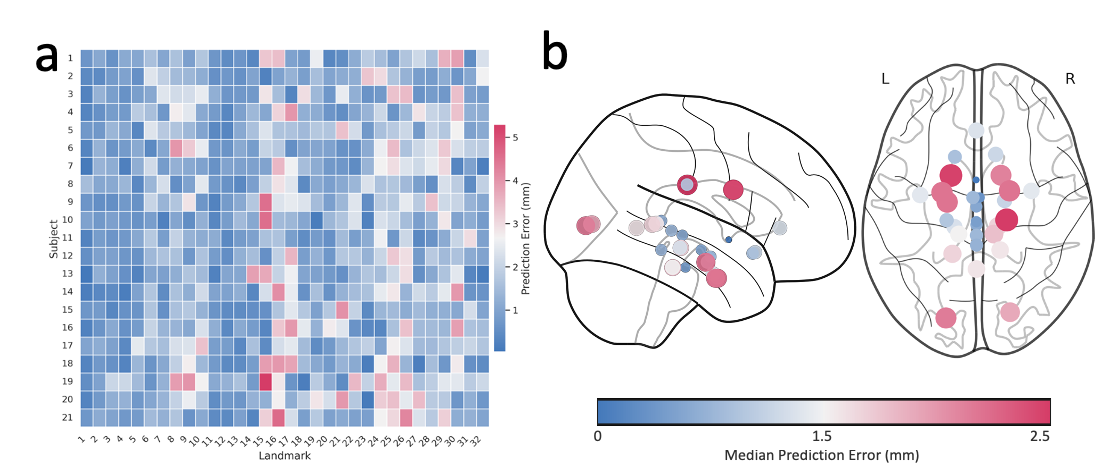
\includegraphics[width=1\linewidth]{figs/ch3_Figure_autoscore.png}
    \caption{Overview of localization error using \texttt{AutoAFIDs}. (a) Heatmap showing Euclidean distance errors (in mm) for each predicted anatomical landmark across 21 test subjects. Each column corresponds to one of the 32 AFIDs, and each row to a subject. (b) Spatial distribution of landmark-specific median prediction errors visualized on a glass brain. Each point represents the anatomical location of an AFID in stereotactic space, with marker size and color encoding the median error across subjects. Higher spatial variability in model accuracy was observed in lateral and ventricular landmarks.}
    \label{fig:ch3_Figure_autoscore}
\end{figure}


Per-landmark performance showed modest variability, reflecting differences in anatomical complexity, tissue contrast, and inter-subject variability. Ten landmarks exhibited median errors in the sub-millimetric range (0.4–0.9 mm), while more challenging regions, such as those adjacent to ventricular structures, demonstrated higher variability (2-2.4 mm). The maximum observed error across all landmarks was 5.28 mm. A complete summary of per-landmark accuracy is provided in Table~\ref{tab:autoafids_accuracy}.


\subsection{Registration Evaluation Using \texttt{AutoAFIDs}}
To assess the sensitivity of \texttt{AutoAFIDs} for evaluating image registration, we compared its predicted landmark coordinates to those derived from \texttt{Lead-DBS} (v3.0; \cite{Neudorfer2023-wd}), a widely used software suite for DBS research that incorporates multi-stage nonlinear registration to align patient MRI data to stereotactic space. In this analysis, we leverage warps generated from \texttt{Lead-DBS} to propagate ground truth AFID annotations on the MNI152NLIN2009b template back to native space.

ED errors were computed across all AFIDs and test subjects, resulting in 672 paired error measurements per method. On average, \texttt{AutoAFIDs} achieved significantly lower localization error (mean: 1.40\,±\,0.85\,mm) compared to \texttt{Lead-DBS} (2.60\,±\,3.19\,mm), with a Wilcoxon signed-rank test confirming statistical significance (\(p < 0.001\)). As shown in Figure~\ref{fig:ch3_Figure_cnnvslead1}a, the error distribution for \texttt{AutoAFIDs} is left-shifted and more tightly clustered, while \texttt{Lead-DBS} displays a heavier tail. Cumulative error curves reinforce this difference, with \texttt{AutoAFIDs} reaching 80\% of data under 2\,mm, compared to only 55\% for \texttt{Lead-DBS}. Figure~\ref{fig:ch3_Figure_cnnvslead1}b shows a scatter plot of the data (i.e., 672 AFIDs) thresholded at 10 mm for visibility. A majority of AFIDs lie above the identity line, indicating superior performance by \texttt{AutoAFIDs}.

\begin{figure}[hbt!]
    \centering
    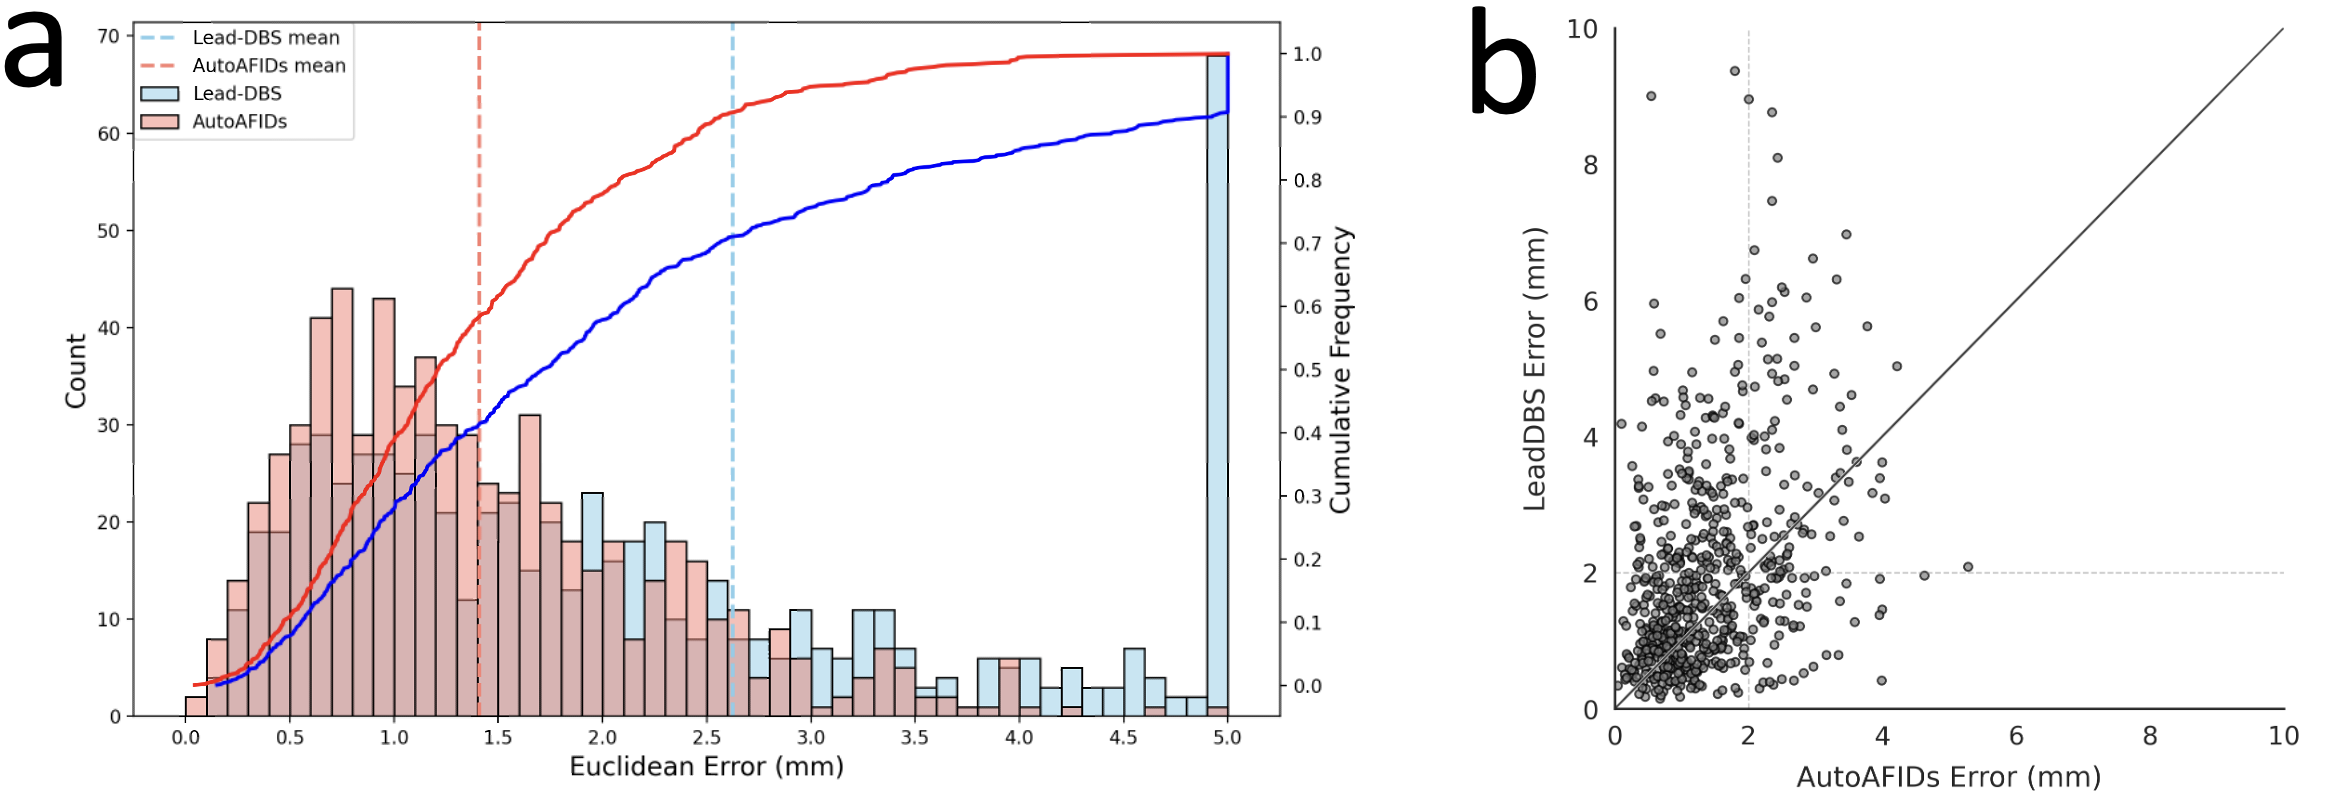
\includegraphics[width=1\linewidth]{figs/ch3_Figure_cnnvslead1.png}
    \caption{Comparison between \texttt{AutoAFIDs} and \texttt{Lead-DBS} at landmark localization in native space. (a) Distribution of all Euclidean distance (ED) for \texttt{AutoAFIDs} (red) and \texttt{Lead-DBS} (blue), shown as overlapping histograms and cumulative frequency curves. Vertical dashed lines indicate means. (b) Scatter plot comparing ED errors for all AFID across all subjects. Each point represents one AFID on a single subject's MRI volume, with the \texttt{AutoAFIDs} error on the x-axis and the corresponding \texttt{Lead-DBS} error on the y-axis. Most points lie above the identity, indicating improved localization accuracy with \texttt{AutoAFIDs} relative to \texttt{Lead-DBS}. The data was thresholded at 10 mm for visibility.}
    \label{fig:ch3_Figure_cnnvslead1}
\end{figure}

To better understand performance differences, we examined both subject-level and AFID-level error patterns using the median ED as a robust measure less sensitive to outliers. Figure~\ref{fig:ch3_Figure_cnnvslead2}a shows paired median EDs for each subject, with the majority demonstrating improved localization accuracy using \texttt{AutoAFIDs}. At the AFID level, Figure~\ref{fig:ch3_Figure_cnnvslead2}b compares median errors across methods, revealing that \texttt{AutoAFIDs} statistically outperformed \texttt{Lead-DBS} on 14 out of 32 AFIDs (\(p < 0.05\)) via a Wilcoxon signed-rank test. These improvements suggest consistent localization advantages, particularly at AFIDs where registration-based methods are more prone to failure.

\begin{figure}[hbt!]
    \centering
    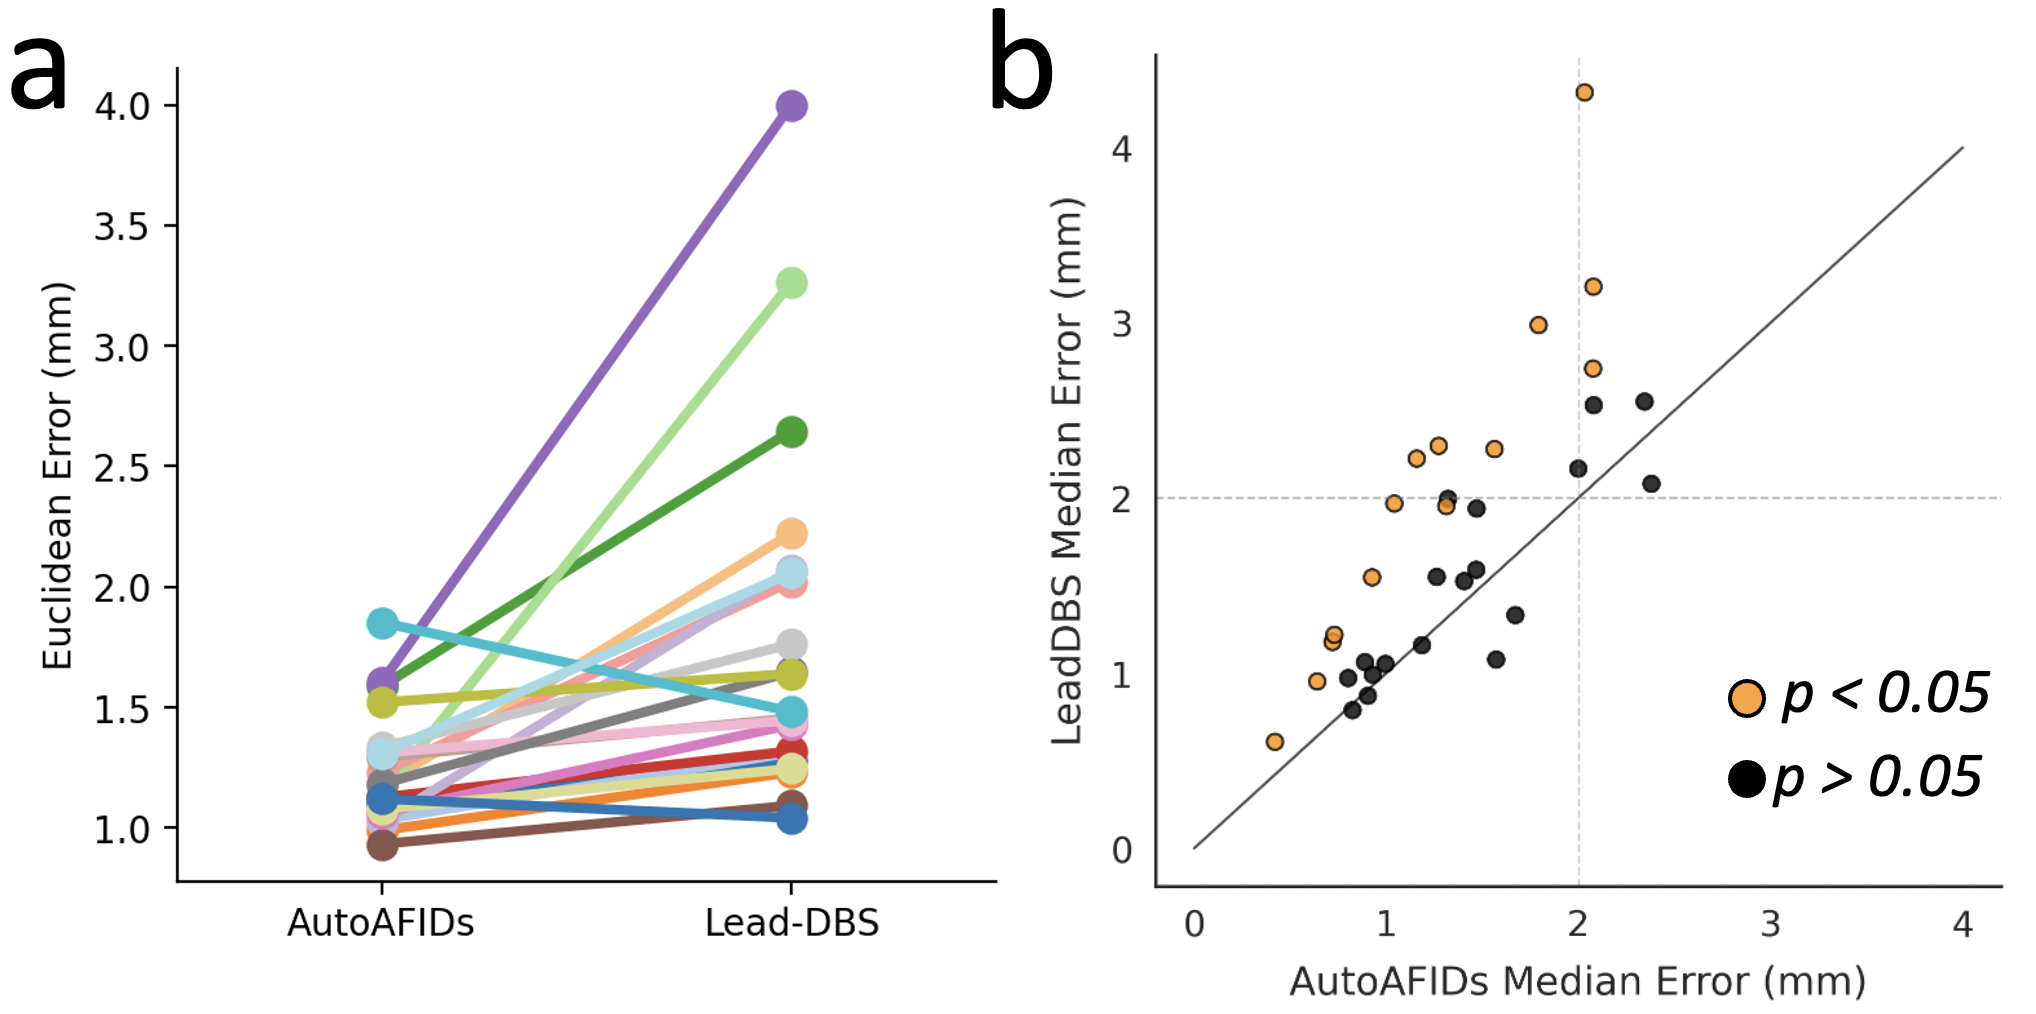
\includegraphics[width=1\linewidth]{figs/ch3_Figure_cnnvslead2.png}
    \caption{Comparison of localization performance between \texttt{AutoAFIDs} and \texttt{Lead-DBS} at the (a) subject and (b) landmark level. (a) Subject-wise median Euclidean distance (ED) errors computed across all 32 landmarks, with most subjects showing lower median error using \texttt{AutoAFIDs}. (b) Landmark-wise comparison of median ED across all subjects. Each point represents one AFID, colored by statistical significance from a Wilcoxon signed-rank test (\(p < 0.05\)), highlighting 14 landmarks where \texttt{AutoAFIDs} significantly outperformed \texttt{Lead-DBS}.}
    \label{fig:ch3_Figure_cnnvslead2}
\end{figure}

Motivated by the variability observed in registration performance, we developed an automated QC application that uses \texttt{AutoAFIDs} coordinate outputs to generate subject-specific summaries of registration accuracy during Lead-DBS analyses. For each subject, our registration QC tool computes descriptive statistics of ED across all 32 AFIDs using deformation warps generated using \texttt{Lead-DBS}. A qualitative review panel presents slice-wise visualizations for each AFID at cardinal planes with crosshairs centered on the registered and reference landmark coordinates. The report also includes a heatmap summarizing localization error by coordinate axis (x, y, z) and a 3D scatterplot visualizing landmark displacement between stereotactic space and the registered subject image. These features enable Lead-DBS users to identify individual landmarks with high registration error, assess global alignment patterns, and quickly spot outliers. A sample report is provided in Figure~\ref{fig:figuresupregqc} with more details on how users can generate these plots in Supplementary section~\ref{app:registrationqualitycontrol}.

\begin{figure}[hbt!]
    \centering
    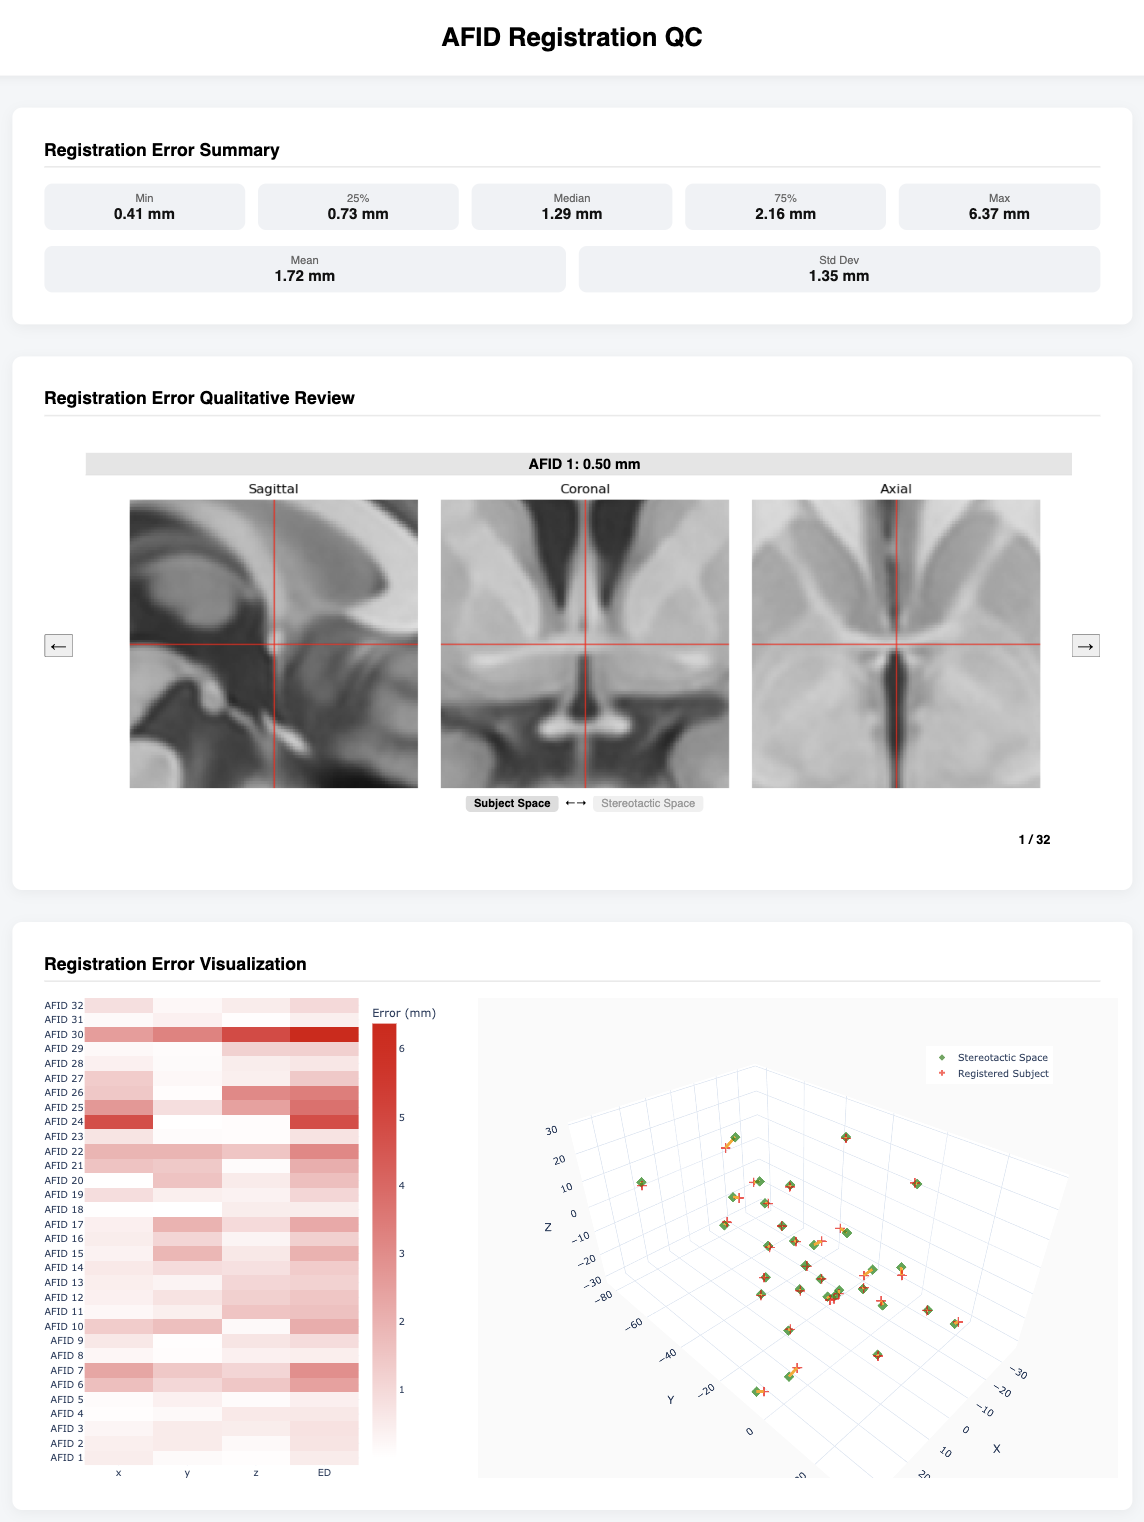
\includegraphics[width=0.80\linewidth]{figs/figuresupregqc.png}
    \caption{Example AutoAFIDs registration quality control report for a subject processed using \texttt{Lead-DBS} \cite{Neudorfer2023-wd}. The subject’s T1-weighted MRI was registered to the MNI152NLIN2009b stereotactic space using default parameters. The resulting \texttt{*.html} file includes: (i) a summary of quantitative error metrics, (ii) qualitative review panels at canonical views cropped around each landmark, and (iii) a landmark-wise error heatmap with 3D visualization of error vectors.}
    \label{fig:figuresupregqc}
\end{figure}

\subsection{Brain Charting Using \texttt{AutoAFIDs}}

To explore how structural brain variability is encoded in pairwise AFID distances (Figure \ref{fig:ch3_Figure_pairwisedata}a), we analyzed a lifespan dataset of 2,834 subjects from nine publicly available neuroimaging cohorts (Figure \ref{fig:ch3_Figure_pairwisedata}b). Subjects ranged in age from 18 to 100 years, with an approximately even sex distribution (50.6\% female; Figure \ref{fig:ch3_Figure_pairwisedata}c) and broad diagnostic coverage (Figure \ref{fig:ch3_Figure_pairwisedata}d), including 2,000 cognitively normal (CN) individuals (70.6\%), 650 with Parkinson’s disease (PD, 22.9\%), and 184 with Alzheimer’s disease (AD, 6.5\%).

\begin{figure}[hbt!]
    \centering
    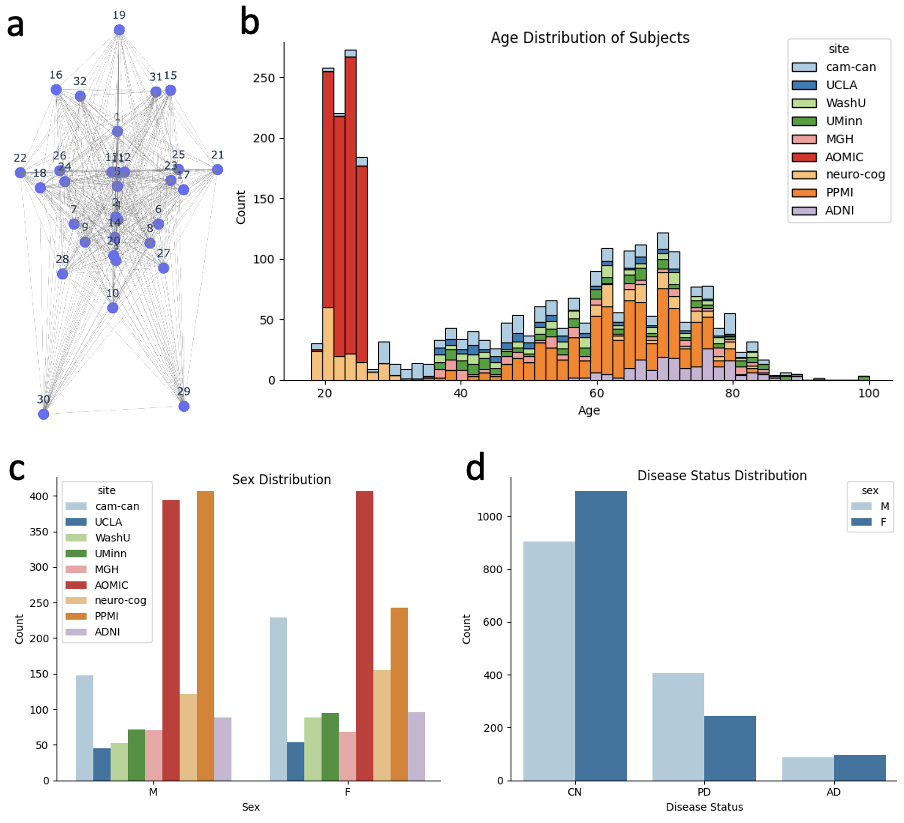
\includegraphics[width=1\linewidth]{figs/ch3_Figure_pairwisedata.png}
    \caption{(a) 3D plot showing all 496 pairwise connections between the 32 anatomical fiducials (AFIDs), illustrating the dense spatial sampling achieved across the brain. (b) Age distribution of subjects stratified by imaging site, demonstrating broad lifespan coverage and diverse dataset contributions. (c) Sex distribution by site, indicating approximate sex balance across most cohorts. (d) Distribution of subjects by disease status and sex, showing that the majority of participants are cognitively normal (CN), with additional representation from Parkinson’s disease (PD) and Alzheimer’s disease (AD) groups.
}
    \label{fig:ch3_Figure_pairwisedata}
\end{figure}

AutoAFIDs annotations were generated for all subjects. We apply a sex- and disease- stratified IQR method to identify and remove outlier subjects based on their mean pairwise AFID distance. Specifically, values falling outside the range \( [Q1 - 3 \times \text{IQR},\ Q3 + 3 \times \text{IQR}] \) were excluded, following Tukey’s rule for detecting extreme outliers.

To investigate morphometric changes more globally, we performed principal component analysis (PCA) to the standardized pairwise distance matrix (i.e., 496 AFID distances) to visualize population-level structure (Figure~\ref{fig:ch3_Figure_PCA}a-d). When colored by sex and age, the PCA revealed a smooth gradient, suggesting that these demographic factors represent principal axes of anatomical variation within the AFID feature space. We observed modest separation by disease status, indicating potential disease-related morphometric signatures. In contrast, no clear clustering was observed by imaging site, suggesting that AFID-based morphometry is relatively robust to differences in image acquisition protocols.
\begin{figure}[hbt!]
    \centering
    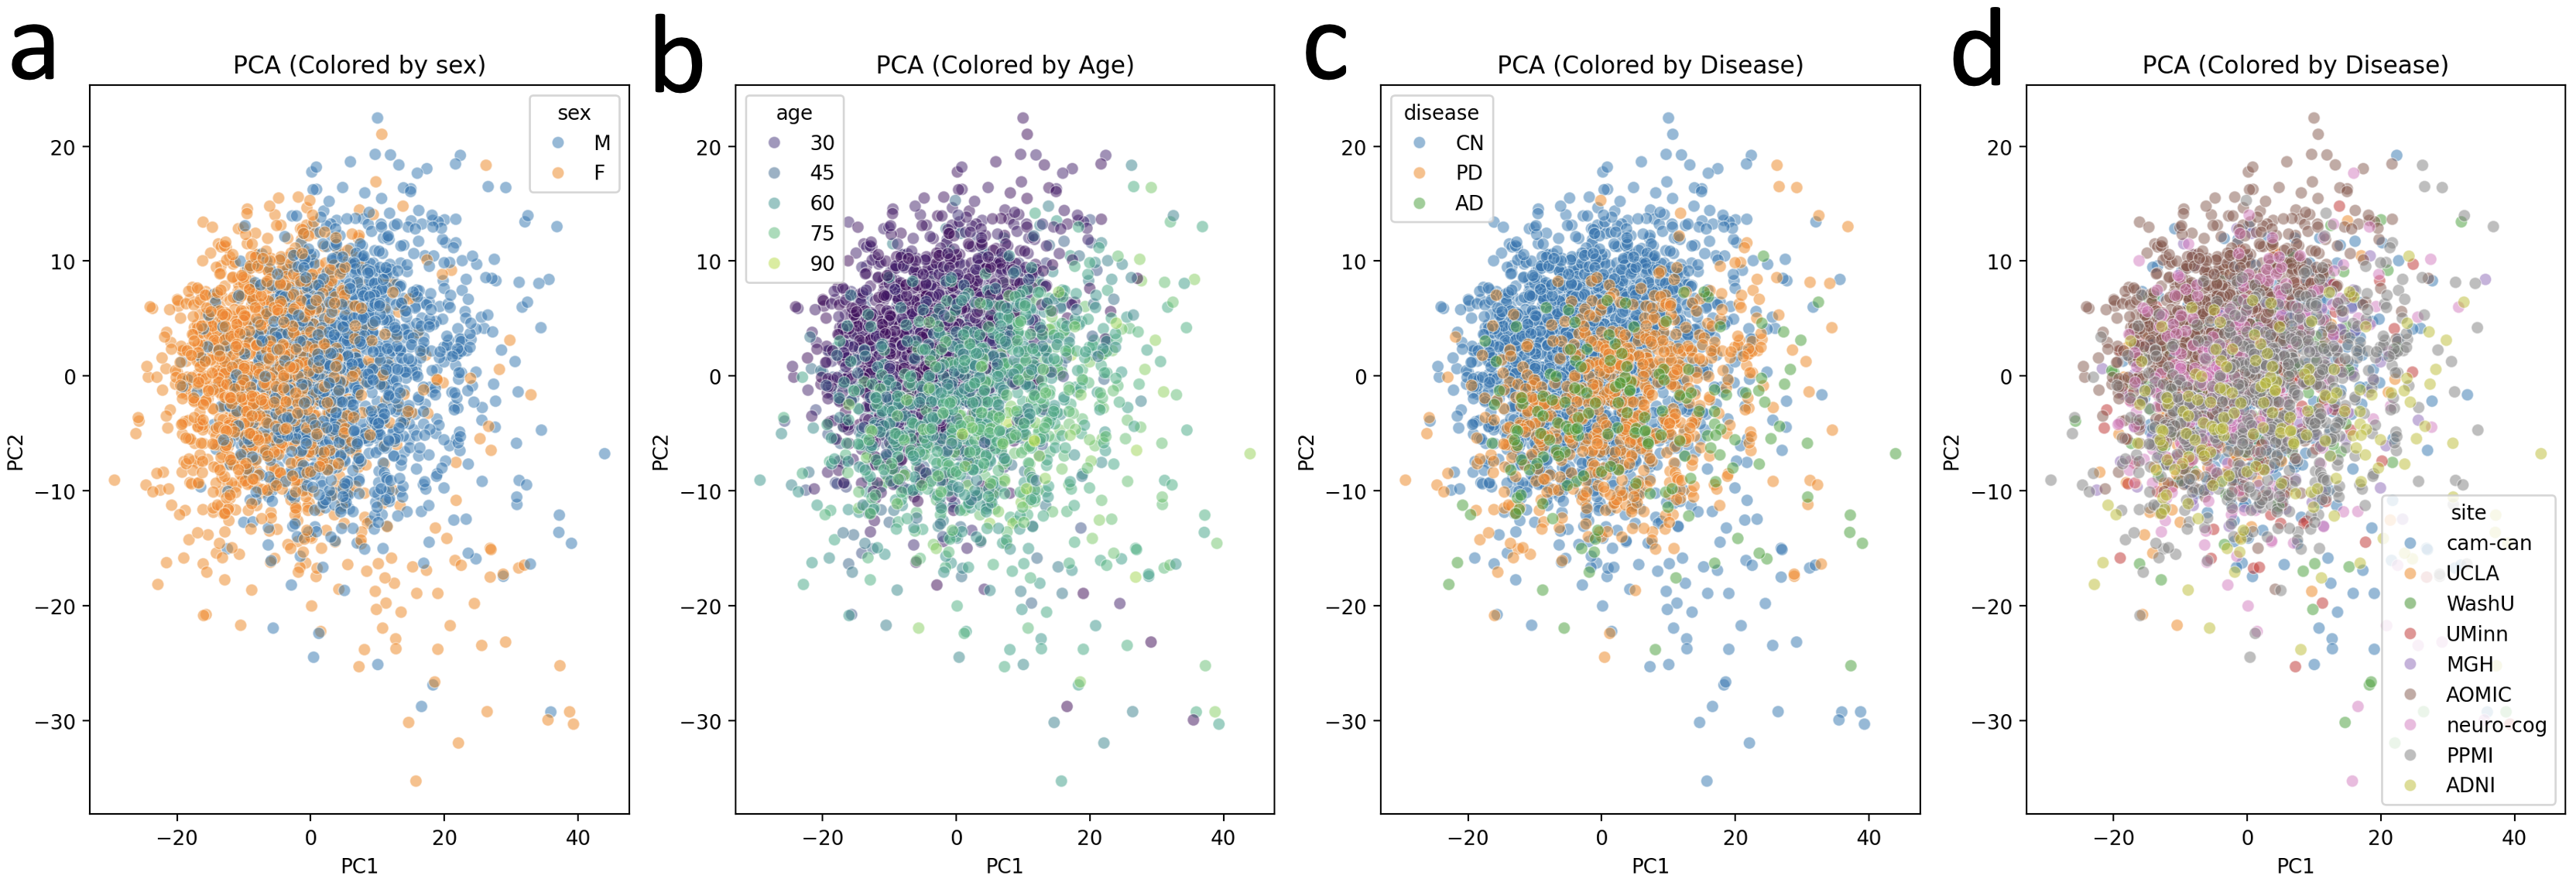
\includegraphics[width=1\linewidth]{figs/ch3_Figure_PCA.png}
    \caption{Principal component analysis (PCA) and age-related correlations in AFID distance space(a–d). Scattr plot of PC1 and P2 projection on standardized AFID pairwise distances. Each point represents a subject and is colored by (a) sex, (b) age, (c) disease status, or (d) acquisition site. A clear gradient is observed along the age axis, while sex, disease, and site show limited separability, suggesting that age is the dominant source of variation in the AFID feature space.}
    \label{fig:ch3_Figure_PCA}
\end{figure}


To examine how specific AFID distances change across lifespan, we computed Pearson correlations between each pairwise AFID distance and age in CN individuals. Figure \ref{fig:ch3_Figure_alldist} shows the global patten in correlations across all the distances. Notably, the majority of the highest negatively correlated distances sample the subcortex with limited spatial representation in the medio-lateral axis. Meanwhile, the majority of the highest positively correlated distances sample the ventricular system and inter-hemispheric distances with limited spatial representation along the anterio-posterior axis. 

\begin{figure}[hbt!]
    \centering
    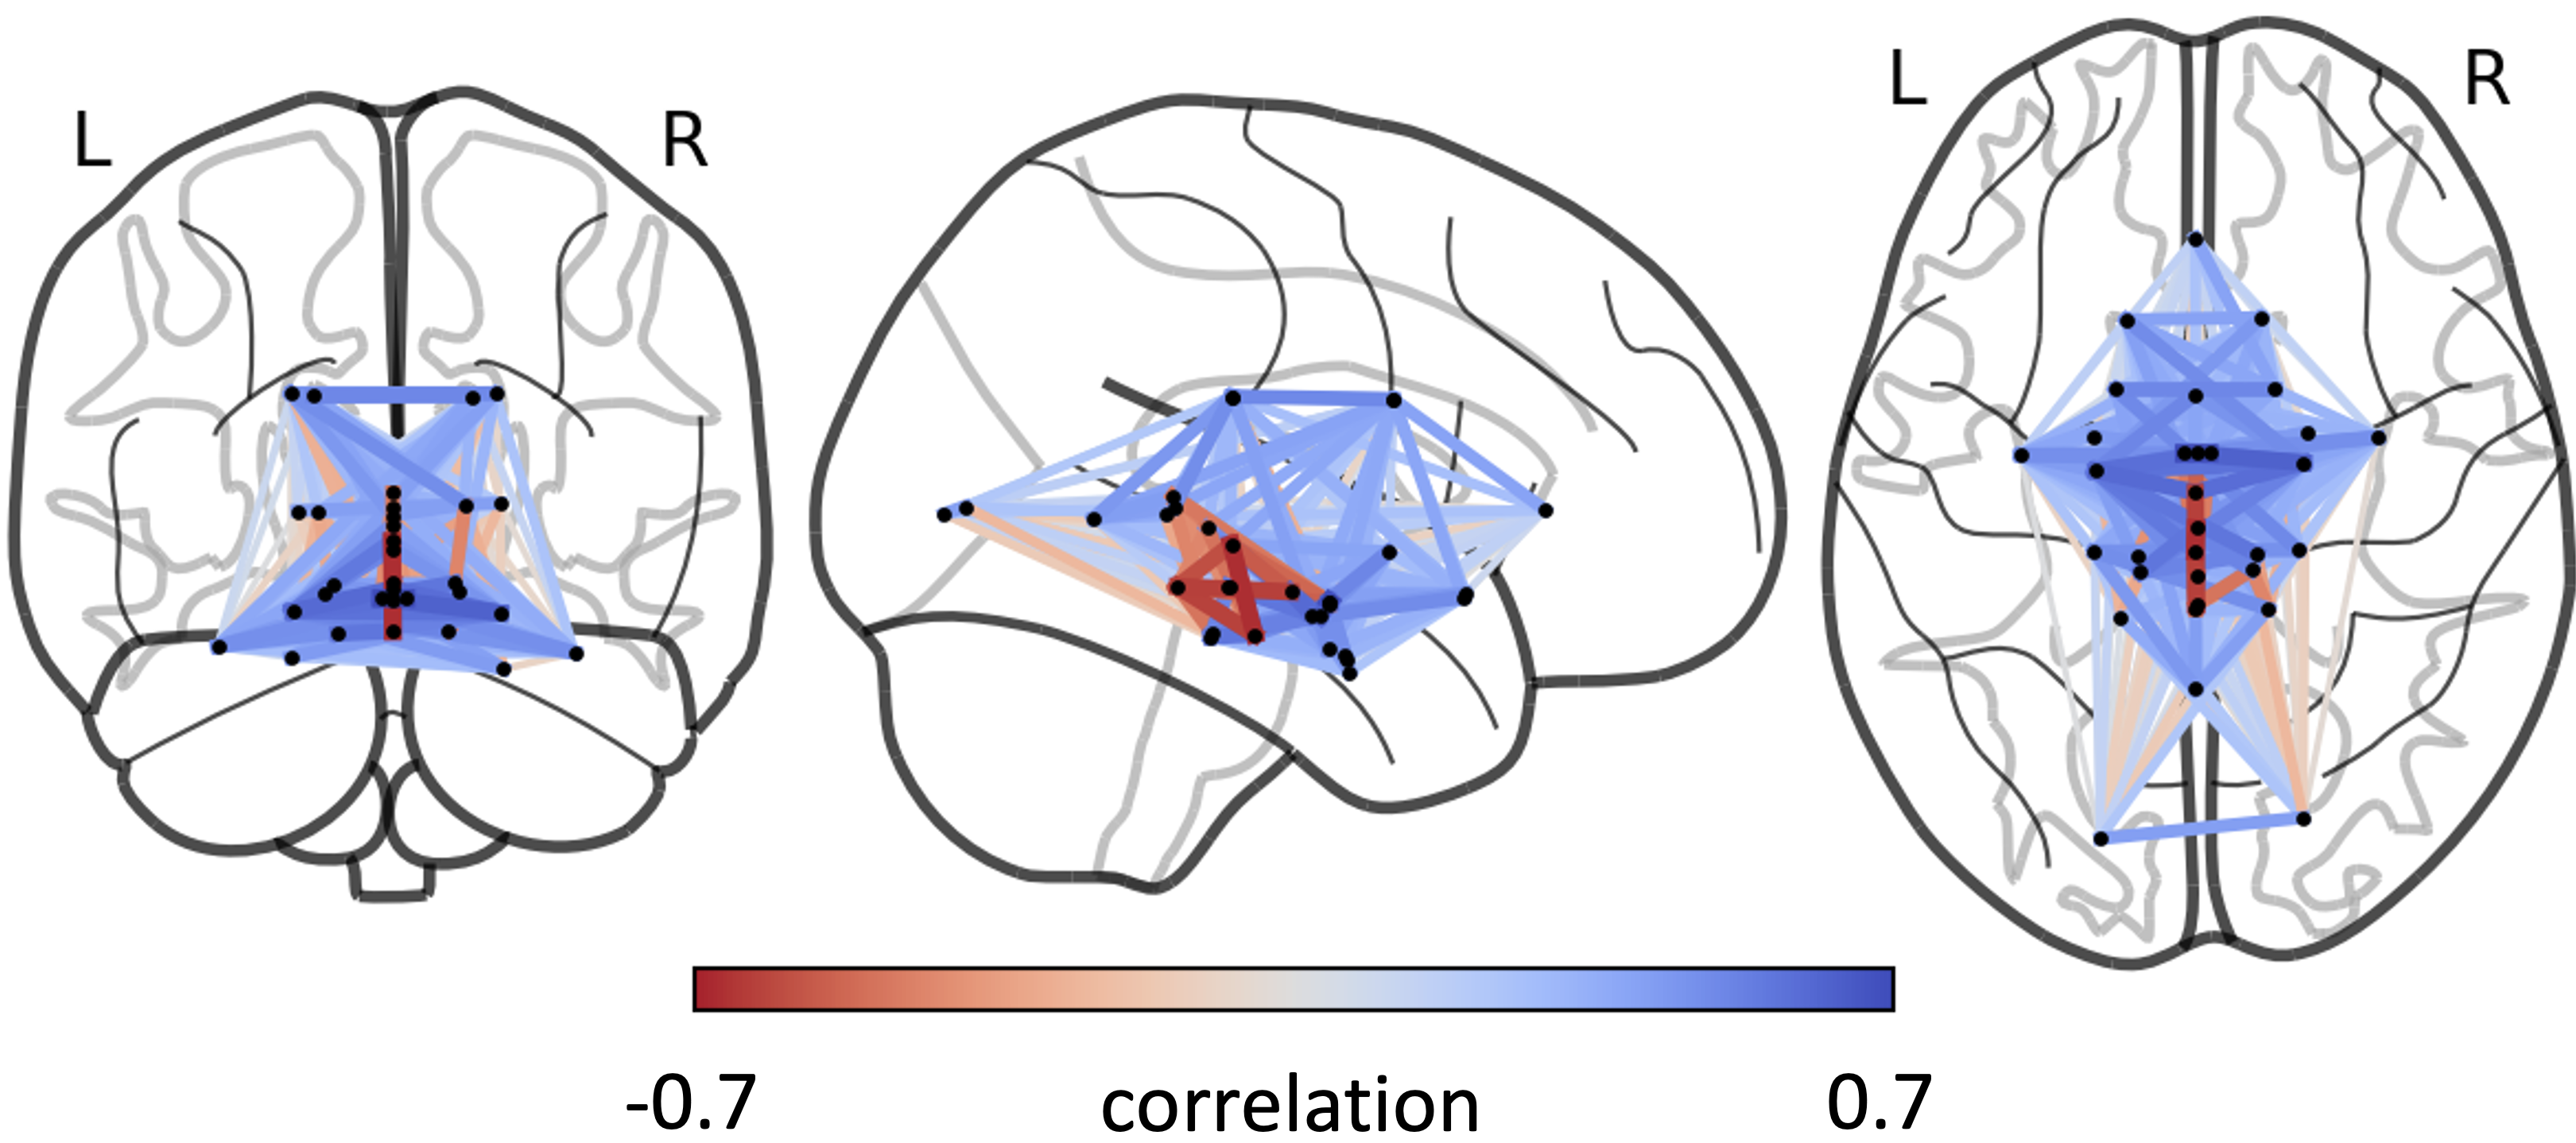
\includegraphics[width=1\linewidth]{figs/ch3_Figure_alldist.png}
    \caption{Age-correlated pairwise anatomical fiducial (AFID) distances. Each edge represents the Pearson correlation between a pairwise AFID distance and age in cognitively normal individuals. Distances that increased with age are shown in shades of blue (positive correlation), while those that decreased are shown in shades of red (negative correlation). Node positions reflect AFID locations in stereotactic space, and views are shown in coronal (left), sagittal (middle), and axial (right) orientations. Notably, positive correlations were concentrated in lateral and periventricular regions (e.g., temporal horns), reflecting expansion with age, whereas negative correlations localized to midline and brainstem landmarks (e.g., infracollicular sulcus and interpeduncular fossa), reflecting age-related compaction.}
    \label{fig:ch3_Figure_alldist}
\end{figure}
To dive deeper into these patterns, we present the top 15 negatively and positively correlated features to age in Figure~\ref{fig:ch3_Figure_tsne}. Several inter- and intra-regional distances demonstrated strong age dependence. The strongest \textbf{negative correlations} involved midline and brainstem-associated structures. The most prominent age-related contractions were observed between AFID~5 and 3 (superior interpeduncular fossa to infracollicular sulcus, $r = -0.70$), AFID~3 and 2 (infracollicular sulcus to posterior commissure, $r = -0.64$), and AFID~5 and 2 (superior interpeduncular fossa to posterior commissure, $r = -0.63$). Additional negatively correlated distances included AFID~11 to 3 (intermammillary sulcus to infracollicular sulcus, $r = -0.55$) and AFID~13 to 3 (right mammillary body to infracollicular sulcus, $r = -0.49$), suggesting coordinated atrophy or compaction within perimesencephalic regions. A consistent pattern emerged involving posterior corpus callosum landmarks as well, including AFID~20 (splenium) to AFIDs~5, 11, 12, and 13 ($r$ values ranging from $-0.46$ to $-0.37$), and nearby midline structures such as AFID~14 (pineal gland) to AFIDs~3 and 5 ($r = -0.45$ and $-0.43$, respectively). These results point to converging evidence of deep midline and diencephalic tissue reorganization with age, particularly in posterior commissural and third ventricular regions.

\begin{figure}[hbt!]
    \centering
    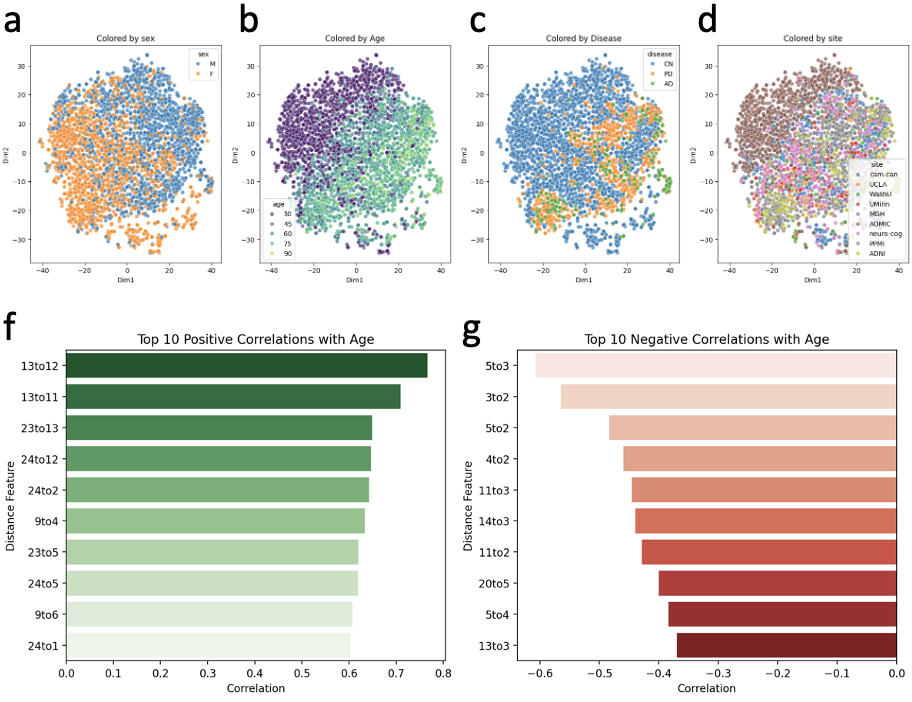
\includegraphics[width=1\linewidth]{figs/ch3_Figure_tsne.png}
    \caption{Age-related correlations in anatomical fiducial (AFID) distance space.(a) and (b) Bar plots showing top 15 AFID pairwise distances with the strongest Pearson correlations with age. (a) Positively correlated distances primarily involve the mammillary bodies and temporal horn fiducials, reflecting expansion of periventricular and CSF spaces with age. Majority of distances are inter-hemispheric representing changes in medio-lateral axis. Furthermore, a subset of positively correlated distances sample ventricular system. (b) Negatively correlated distances involve brainstem and midbrain fiducials, potentially reflecting age-related compaction or atrophy along the brainstem axis. All of the top 15 pairwise distances correlated with age are in the brainstem and mostly span the anterior posterior axis. 
    }
    \label{fig:ch3_Figure_tsne}
\end{figure}

The strongest \textbf{positive correlations} were observed between anterior and medial temporal structures. Notably, distances between AFID~23 (left superior anteromedial temporal horn) and AFID~13 (right mammillary body) showed the highest correlation with age ($r = +0.58$), followed closely by AFID~23 to 5 (left superior anteromedial temporal horn to superior interpeduncular fossa, $r = +0.55$), and AFID~24 to 12 (right superior anteromedial temporal horn to left mammillary body, $r = +0.54$). Additional features included inter-ventricular and peritemporal expansions, such as AFID~24 to 6 (right superior anteromedial temporal horn to right superior lateral mesencephalic sulcus, $r = +0.52$) and AFID~23 to 11 (left superior anteromedial temporal horn to intermammillary sulcus, $r = +0.50$). Many of these correlated features involve AFIDs~23 and 24, which anchor the temporal horns, highlighting the role of ventricular enlargement and limbic expansion as primary morphological signatures of aging.

We further examined age-related changes in the anterior commissure–posterior commissure (AC–PC) distance, given their central role as key landmarks in stereotactic neurosurgery. Across CN individuals, we observed a small but consistent increase in AC–PC length with age in both males and females (Figure~\ref{fig:ch3_Figure_acpc}). Males had longer AC–PC distances than females (median ± IQR: 26.63 ± 1.48 mm vs. 25.81 ± 3.04 mm, respectively). In the PD subgroup, AC–PC distances were generally longer than in cognitively normal individuals. Males also had a longer AC-PC distance than females, median of 28.22 ± 5.14 mm vs. 27.25 ± 3.76 mm, respectively. To account for potential confounding by age, we matched comparisons of AC–PC distance between CN and PD groups. Even after matching, AC–PC distances remained significantly longer in the PD group (p \(<\) 0.001) via Mann-Whitney U test, suggesting disease-associated structural changes along this canonical axis. This reinforces the relevance of individualized targeting in stereotactic applications where the AC–PC line serves as an anatomical reference.

\begin{figure}[hbt!]
    \centering
    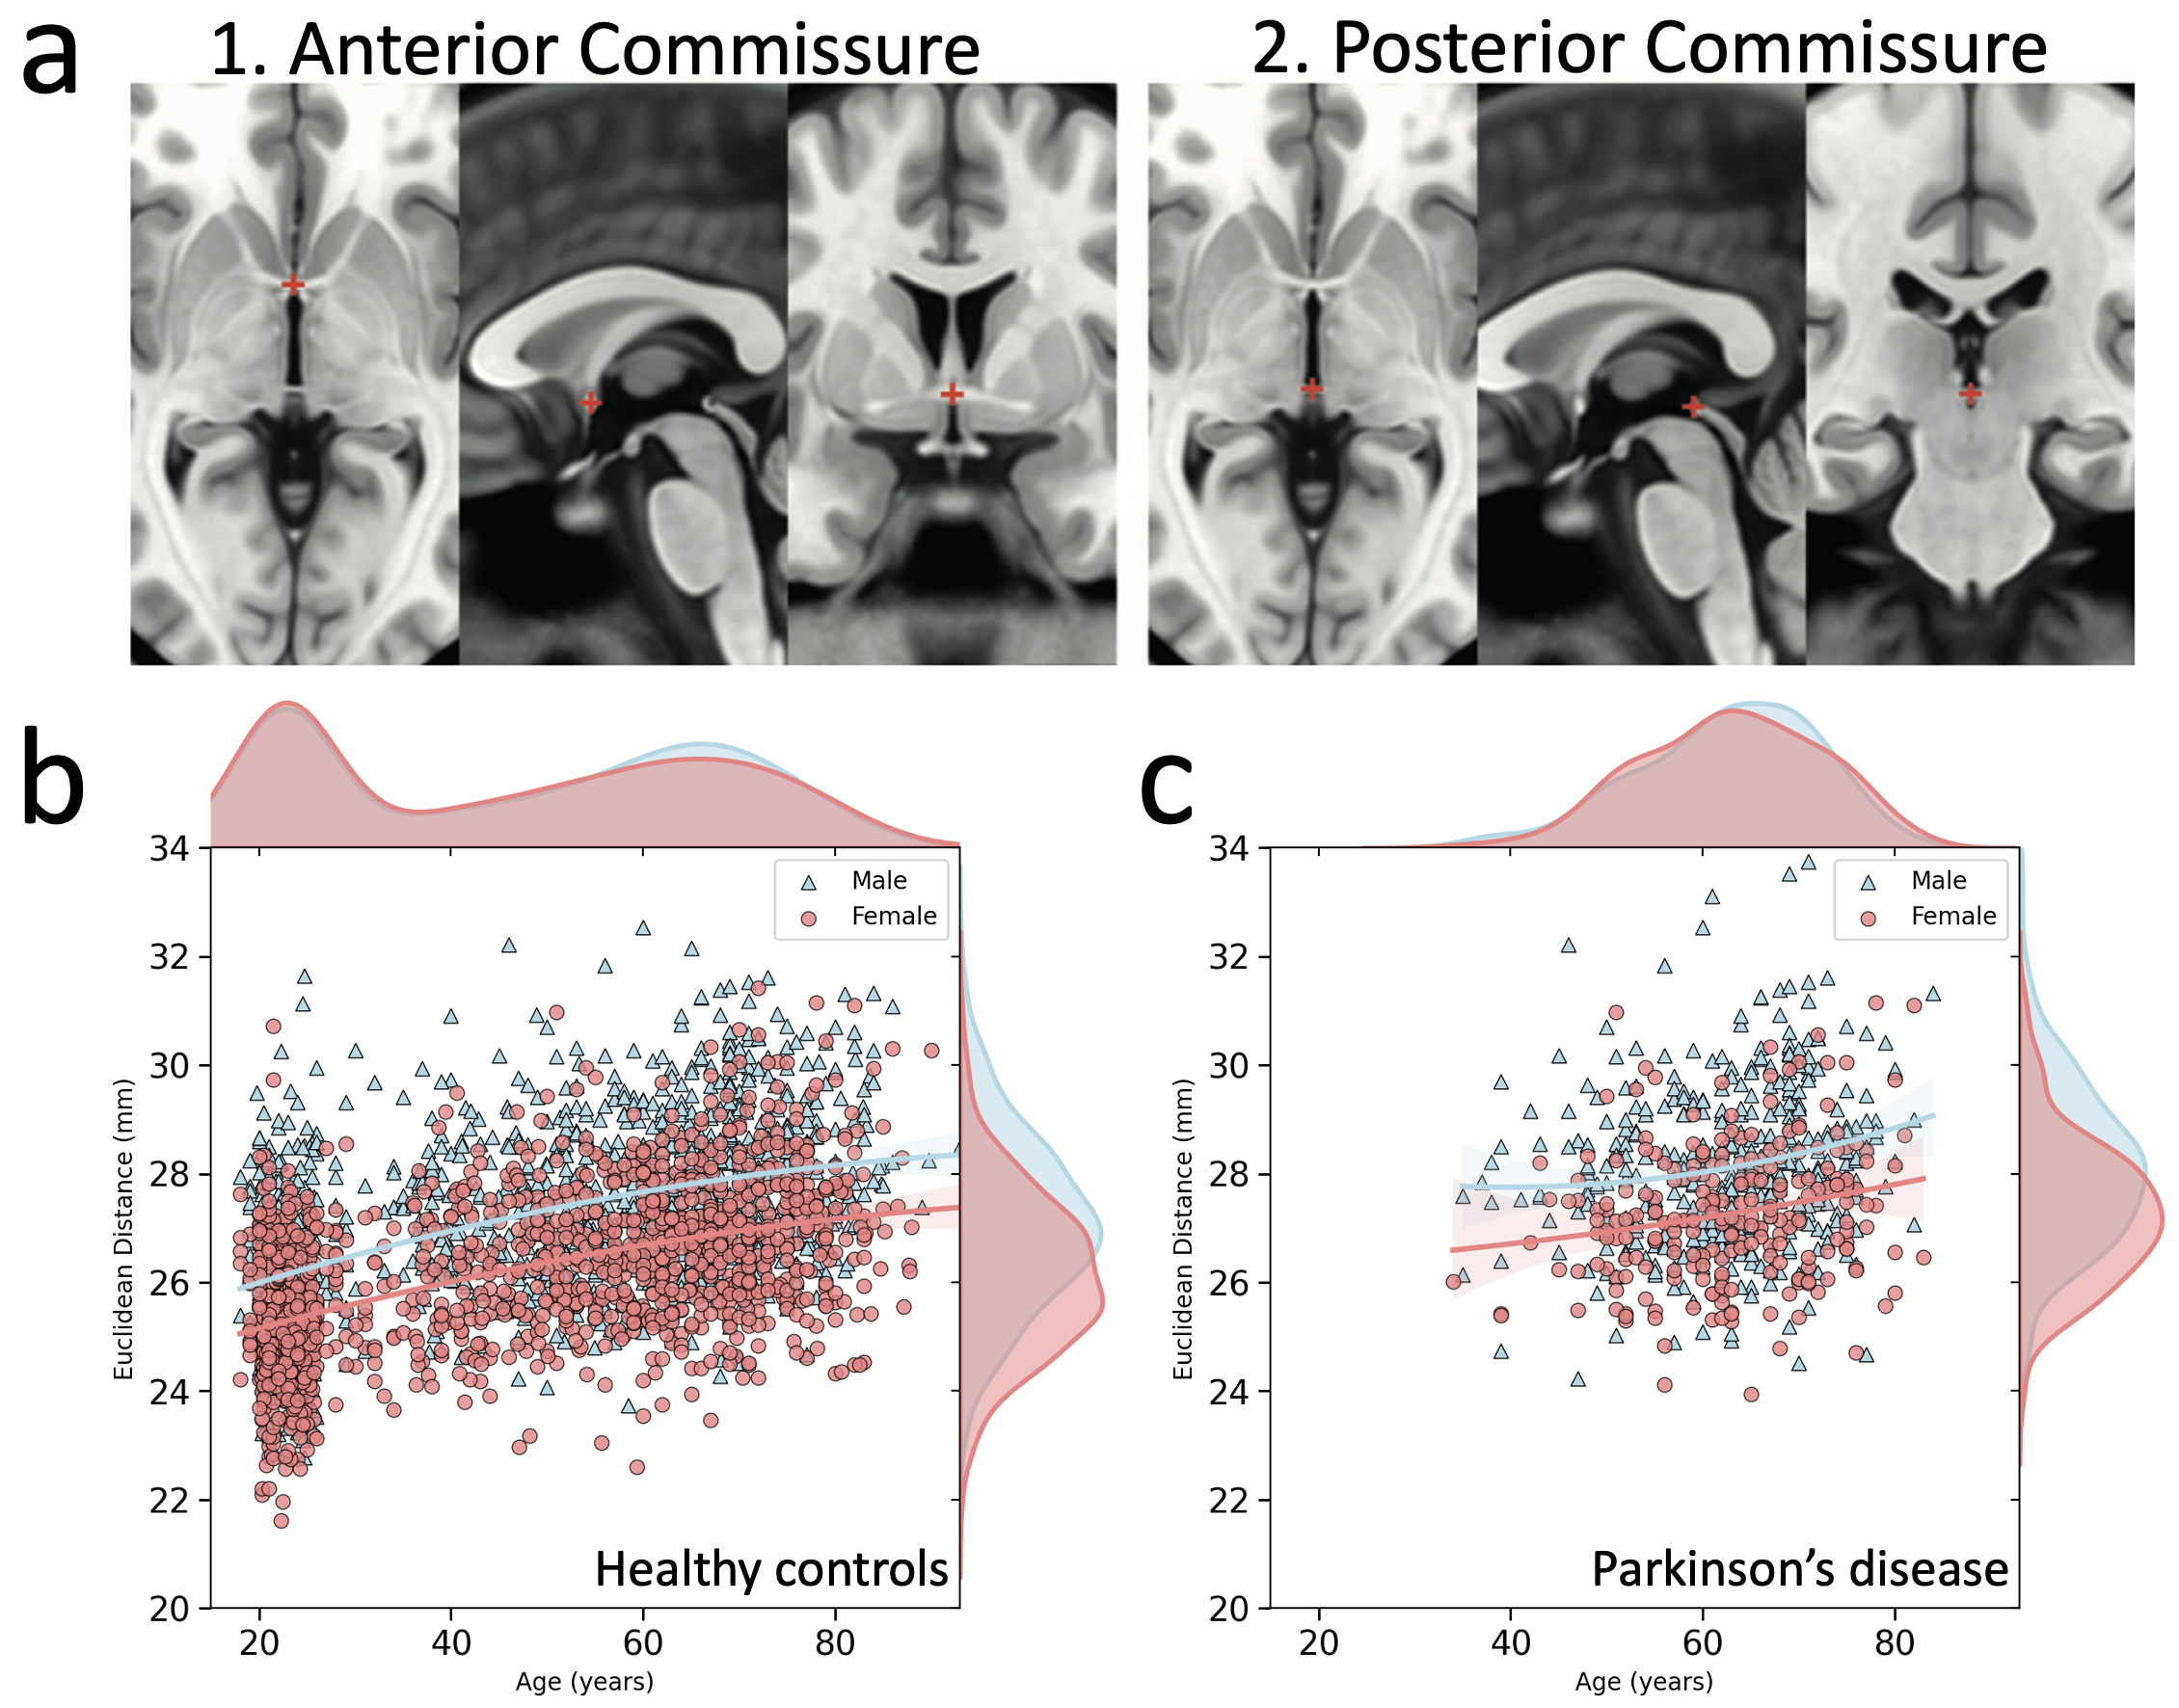
\includegraphics[width=1\linewidth]{figs/ch3_Figure_acpc.png}
    \caption{Anterior commissure–posterior commissure (AC–PC) line across age and disease. (a) Anatomical definition of the AC (left) and PC (right) shown in canonical views. (b) Age-related trends in AC–PC distance among cognitively normal cohort. A subtle increase in distance is observed with age, with males showing longer distances than females. (c) AC–PC distances in individuals with Parkinson’s disease. A similar age-related trend is observed. Shaded bands represent 95\% confidence intervals for sex-stratified second-order polynomial fits.
    }
    \label{fig:ch3_Figure_acpc}
\end{figure}
\section{Discussion}
In this study, we introduce \texttt{AutoAFIDs}, an open-source deep learning-based framework for automatic localization of anatomical fiducials (AFIDs) with millimetric accuracy. Our data and code is designed for generalizability, enabling incorporation into various software compatible with the BIDS specification. \texttt{AutoAFIDs} can quality control registration and capture morphometric changes in the human brain. This work introduces a novel framework for stereotactic brain charting across the human lifespan, which we leverage to characterize morphometric changes in healthy aging and neurodegenerative disease.

\subsection{Landmark Localization Performance}

\texttt{AutoAFIDs} achieved a median Euclidean distance (ED) of 1.21 mm (IQR: 0.76–1.95 mm) across 32 AFIDs in a held-out test set of 21 subjects. These results are in line with the range reported for similar tasks \cite{Ertl2025-wu, Salari2024-iu, Edwards2021-su} and approach expert-level precision (0-2 mm), particularly for brainstem landmarks \cite{Abbass2022-lf}. Ten of the 32 AFIDs showed sub-millimetric median errors, while more anatomically variable regions, such as those near the ventricles, exhibited higher variability. This was also consistent with prior reports of inter-rater localization accuracy \cite{Lau2019-eh, Abbass2022-lf}. Although we did not perform a direct comparison between \texttt{AutoAFIDs} and inter-rater localization accuracy, we direct the reader to Chapter \ref{chap:afidsdata} where we provide a breakdown of inter-rater localization accuracy across all AFID datasets. 

Several competing models for landmark localization in brain MRI offer direct points of comparison, as they make use of the AFIDs data released in Chapter~\ref{chap:afidsdata}. Among them, \texttt{nnLandmark} \cite{Ertl2025-wu} reported an average localization error of approximately 1.27 mm. However, accuracy per landmark was not reported, limiting insight into how the model performs across anatomically diverse regions, particularly in challenging areas near the ventricular system. Given that \texttt{nnLandmark} also employs a U-Net architecture, the overall similarity in accuracy to \texttt{AutoAFIDs} is expected. A notable limitation in \texttt{nnLandmark} is the lack of a released codebase and the absence of compatibility with the BIDS specification. This increases the technical burden for neuroimaging researchers and developers, who must independently integrate model inference into large-scale, BIDS-compliant workflows. Another landmark localization model, \texttt{DeepNavNet} \cite{Edwards2021-su}, which uses a 3D residual network architecture, focuses on localizing the anterior and posterior commissure (AC and PC) for neuronavigation. \cite{Edwards2021-su} reported localization errors of 0.79 ± 0.33 mm and 0.78 ± 0.33 mm for the AC and PC respectively. These results are comparable to the performance of \texttt{AutoAFIDs} for the same landmarks (AC: 0.42 mm, PC: 0.83 mm), demonstrating competitive accuracy even relative to models and network architectures specialized for only two targets. In contrast, \cite{Salari2024-iu} developed \texttt{CABLD}, a contrast-agnostic self-supervised approach to landmark regression that involves only annotating a single reference example. While this flexibility is notable, the reported accuracy of \texttt{CABLD} is on the order of 3–4 mm. This level of performance is insufficient for millimetric applications such as registration quality control, where we show that even established nonlinear pipelines like \texttt{Lead-DBS} achieve average landmark alignment errors on the order of 1-3 mm. The lower accuracy of \texttt{CABLD}, therefore, restricts its utility in cases where a high level of precision is required.

A key strength of \texttt{AutoAFIDs} lies in the design of the system, where each landmark is treated as a separate supervised learning task with its own dedicated model. This modular, per-landmark approach allows new anatomical targets to be easily added to the framework without retraining the entire system. It also enables more tailored optimization for each landmark, which may be especially important for landmarks with distinct spatial or contrast features. Another advantage of \texttt{AutoAFIDs} is its modular and user-facing configuration (see Supplementary content~\ref{app:yaml}), which is compatible with the BIDS specification. To our knowledge, no current BIDS-aware tools exist in the literature for brain landmark localization. This flexibility, combined with consistent sub-millimetric to low-millimetric accuracy, positions \texttt{AutoAFIDs} as a scalable tool for brain mapping and surgical planning.

\subsection{Evaluation of Registration Accuracy}

To validate that \texttt{AutoAFIDs} can provide a meaningful and millimetric registration quality control reports, we benchmarked it against \texttt{Lead-DBS}. \texttt{AutoAFIDs} significantly outperformed \texttt{Lead-DBS} on landmark localization accuracy across subjects and AFIDs (p\(<\)0.001), with statistically superior performance in 14 of 32 landmarks. These results validate that \texttt{AutoAFIDs} can provide the needed sensitivity for quality control. It is important to note that \texttt{Lead-DBS} employs a rigorously validated registration scheme and was curated by comparisons of six modern and established algorithms \cite{Ewert2019-cc}. Thus, \texttt{Lead-DBS} serves as a strong benchmark for comparison, though it may overestimate the performance of general-purpose in-house registration tools. Beyond group-level accuracy, \texttt{AutoAFIDs} also provides a valuable framework for registration quality control by generating intuitive, subject-specific visualizations and quantitative error summaries. To our knowledge, no existing open-source tools offer automatic and reproducible quantitative metrics for evaluating registration accuracy; most neuroimaging software still relies on qualitative visual inspection. By enabling the detection and quantification of misalignments, \texttt{AutoAFIDs} promotes greater transparency and accountability in image preprocessing—an increasingly important consideration as neuroimaging and neurosurgical workflows become more reliant on automated pipelines.

\subsection{Structural Brain Charting Across the Lifespan}
We demonstrated that AFID pairwise distances automatically predicted using \texttt{AutoAFIDs}, capture meaningful structural variation across the human lifespan and provide a robust framework for population-level morphometric analysis. By analyzing 2,834 MRIs from nine diverse public neuroimaging cohorts, we show that coordinate-based representations of brain anatomy can encode individual differences related to age, sex, and disease status, while remaining resilient to variability in imaging site and acquisition protocol. While recent brain charting efforts \cite{Bethlehem2022-ow,Di-Biase2023-nv} have focused on global or regional measures such as total brain volume, cortical thickness, or subcortical structure size, our approach here offers a complementary geometric perspective by characterizing inter-landmark distances across standardized anatomical landmarks.

\subsection{PCA Morphometric Patterns}
Dimensionality reduction via PCA revealed that age and sex are principal axes of variation in the AFID-derived feature space, consistent with prior studies that report global and regional brain volume changes associated with these demographic factors \cite{Fjell2010-aq, Ritchie2018-df}. The continuous age gradient observed in PCA space indicates that AFID pairwise distances encode smooth anatomical changes across the lifespan, likely reflecting progressive atrophy, ventricular expansion, and sulcal widening. Notably, the minimal clustering by acquisition site supports the modality-agnostic potential of this framework, underscoring its utility for multi-cohort studies where scanner variability often confounds traditional voxelwise analyses \cite{Fortin2018-ke}.

Limited disease-specific differentiation in PCA space suggests that while coordinate-based features are sensitive to broad morphometric changes, finer-grained modeling may be necessary to uncover disease-related patterns. However, the modest separation of Parkinson’s disease (PD) and Alzheimer’s disease (AD) subjects from cognitively normal individuals in some regions of the PCA space hints at latent structure that could be further disentangled using supervised classification or longitudinal modeling. Importantly, the minimal influence of acquisition site variability confirms that the AFID-based feature space may generalize well to clinical datasets collected across institutions, an essential property for developing robust disease biomarkers.

\subsection{AFID-pairwise Distance and Age Correlations}
Our correlation analysis within cognitively normal individuals revealed distinct anatomical changes across the lifespan. Notably, AFID distances that negatively correlated age were concentrated in midline subcortical regions, particularly involving the brainstem and diencephalon. This is consistent with established findings of early and progressive shrinkage in subcortical volume with age, especially the midbrain, pons, and posterior commissural system, as shown in volumetric and voxel-based morphometry studies \cite{Dima2022-dp, Raz2005-jr}. Importantly, our results localize these changes to compact midline structures (e.g., infracollicular sulcus, interpeduncular fossa, and posterior commissure), providing finer spatial resolution than previous global or lobar approaches. Conversely, AFID distance that positively correlated with age primarily involved lateral, periventricular structures such as the mammillary bodies and temporal horn fiducials. These patterns are in line with age-related expansion of cerebrospinal fluid (CSF) spaces and ventricular enlargement, which have been well-documented as sensitive biomarkers of neurodegeneration and normal aging \cite{Fujita2023-vi,Resnick2003-je,Bethlehem2022-ow}. Importantly, the inter-hemispheric and medio-lateral expansion observed in our data reflects symmetric CSF redistribution and loss of parenchymal volume in periventricular white matter regions, consistent with prior longitudinal studies \cite{Fujita2023-vi,De-Vis2016-li}. Our findings here broadly align with recent large-scale analyses of neuroanatomical trajectories across the lifespan. For instance, \cite{Bethlehem2022-ow} charted normative brain development using over 100,000 MRI scans and reported volumetric decline in brainstem regions alongside prominent ventricular expansion—paralleling the dual trajectory evident in our AFID-based analysis. Crucially, our method captures these dynamics using anatomical landmarks, suggesting that AFID-based morphometry can serve as a low-dimensional yet sensitive proxy for detecting coordinated structural brain changes.

\subsection{Clinical Relevance of the AC–PC Line}
Given its central role in neurosurgical targeting, we analyzed the anterior commissure–posterior commissure (AC–PC) distance---a canonical stereotactic reference axis. In cognitively normal individuals, we observed a subtle but consistent increase in AC–PC length with age, as well as longer distances in males compared to females. These findings align with prior reports that link AC–PC length to demographic variation, including age- and sex-associated neuroanatomical changes \cite{Lee2008-nd}. Our analysis also revealed that patients with PD exhibited significantly greater AC–PC distances than age-matched controls. This observation is consistent with a prior studies by \cite{Lee2008-nd,Dabadi2020-am}. Importantly, traditional stereotactic systems often rely on standardized templates or fixed AC–PC-based reference coordinates. Our findings reinforce the necessity of individualized anatomical localization to ensure accurate DBS targeting. By enabling automated and precise identification of stereotactic landmarks, \texttt{AutoAFIDs} provides a scalable solution to incorporate subject-specific geometry into surgical planning.

\subsection{Limitations and Future Directions}

In this work, we have shown \texttt{AutoAFIDs} to consistently locate anatomical landmarks with milimetric precision and have demonstrated its downstream applications in neuroimaging research and neurosurgical planning. However, several limitations should be acknowledged to contextualize these results and guide future directions.

Our model was trained using AFID annotations avergaed from multiple raters. While these annotations followed a standardized protocol, inter-rater variability remains an inherent source of error especially in regions with poor tissue contrast leading to difficulty in clearly defining anatomical boundaries. Prior work has shown that even among trained raters, millimetric discrepancies in annotations are common in ventricular and subcortical regions \cite{Lau2019-eh,Abbass2022-lf}, which may impose an upper bound on the maximal accuracy of our supervised model. We did not incorporate strategies such as multi-rater fusion, probabilistic ground truths, or weak supervision \cite{Salari2024-rw} that have been shown to improve robustness and uncertainty modeling in landmark detection. Future versions of \texttt{AutoAFIDs} may benefit from integrating these strategies to better handle annotation uncertainty and increase model reliability.

The 3D U-Net architecture underlying \texttt{AutoAFIDs} enabled accurate localization of our selected AFIDs, but it may not be optimal for all types of anatomical landmarks. Alternative architectures, such as attention-based networks or models inspired by YOLO \cite{Redmon2015-ia}, have demonstrated state-of-the-art performance in object detection tasks. However, these models typically require more complex training regimes, greater computational resources, and are not as widely adopted in 3D medical imaging pipelines. Our decision to use a U-Net was motivated by its established performance in 3D medical image segmentation \cite{Cicek2016-dz}, ease of integration with 3D patch-based training, and its competitive accuracy compared to inter-rater variability. Future work may explore hybrid or attention-enhanced architectures to improve landmark resolution, particularly in morphologically heterogeneous regions.

To enhance generalizability beyond T1-weighted inputs, we employed SynthSR \cite{Iglesias2023-co}, a widely used domain-adaptive tool that synthesizes 1~mm isotropic MP2RAGE-like volumes from various input modalities (e.g., T2w, FLAIR, CT). While this enables broader applicability of \texttt{AutoAFIDs} in various contexts where high-resolution T1w images may be unavailable, SynthSR has not been explicitly validated for millimetric accuracy in stereotactic applications. As such, we include warnings in the software documentation advising caution when applying the model to non-T1w modalities and encourage users to visually inspect results. Rigorous validation of SynthSR-based inference remains an important future direction, particularly as synthetic image pipelines gain traction in neurosurgical planning.

Finally, although we presented initial analyses of brain morphometry and disease-related variability using \texttt{AutoAFIDs}, these were intended as proof-of-concept demonstrations. The curated dataset enables a much deeper exploration of anatomical differences across lifespan and disease states, including longitudinal and progression-related changes. We view this work as the first step in that direction, and future studies will leverage \texttt{AutoAFIDs} to more systematically investigate these questions.

In summary, \texttt{AutoAFIDs} provides a strong foundation for accurate and interpretable landmark localization, but future work will benefit from exploring architectural advances, modality-specific refinements, and large-scale morphometric modeling to realize its full potential.

\section{Conclusion}

\texttt{AutoAFIDs} offers a generalizable, high-accuracy tool for automatic anatomical landmark localization. Its ability to detect subtle structural variation, assess registration quality, and enable coordinate-based brain morphometry opens new possibilities for scalable, interpretable, and individualized neuroimaging analysis. As interest in reproducible and large-scale neuroimaging grows, \texttt{AutoAFIDs} can serve as a tool toward quality control and advancing precision brain mapping.



